\documentclass[11pt]{article}
\usepackage[letterpaper,margin=.25in]{geometry}
\usepackage{amsmath,amssymb,booktabs,array,tabularx,xcolor,tikz,hyperref,embedfile,microtype}
\usetikzlibrary{trees}
\hypersetup{colorlinks=true,urlcolor=blue!55!black}
\pagestyle{empty}
\setlength{\parindent}{0pt}
\setlength{\parskip}{4pt}
\linespread{1.035}\selectfont
\definecolor{navy}{RGB}{25,54,86}
\definecolor{soft}{RGB}{244,247,250}
\tikzset{branch/.style={circle,draw=navy,line width=.6pt,inner sep=2pt},trueleaf/.style={circle,draw=navy,fill=navy,inner sep=2.1pt},falseleaf/.style={circle,draw=navy,fill=white,inner sep=1.8pt}}
\newcommand{\sectionbar}[1]{\vspace{3pt}{\color{navy}\bfseries #1}\par\vspace{2pt}\hrule\vspace{4pt}}
\begin{document}
\enlargethispage{.12in}

\embedfile[desc={A120599 exact certificate payload},mimetype=application/json]{certificate_payload.json}
{\color{navy}\LARGE\bfseries A120599 concise calculus certificate}\hfill{\small VERIFIED}\\[-1pt]
{\small Bradley Klee, \quad Mech.An.ika Sol (Open AI) \hfill July 31, 2026}

\sectionbar{Definition and first terms}
\(\displaystyle 13\,A(x)=12+32\,x+A(x)^{5}\), with the origin-normalized solution.\\
{\footnotesize Normalization/grammar: \texttt{A(x)=1+(4)*T(x); T=x+5*T\textasciicircum{}2+20*T\textasciicircum{}3+40*T\textasciicircum{}4+32*T\textasciicircum{}5}.}\\
\(a(0),\ldots,a(7)=1,4,20,280,4660,86728,1727880,36047280\).\\[2pt]
{\small Kernel used throughout: \(\displaystyle \rho(u)=u\,(1-5\,u^{1}-20\,u^{2}-40\,u^{3}-32\,u^{4})\), so \(x=\rho(T(x))\).}

\sectionbar{Typogeometry}
\begin{minipage}[t]{.235\textwidth}\centering 
\begin{tikzpicture}[level distance=9mm,level 1/.style={sibling distance=10mm},level 2/.style={sibling distance=6mm},scale=.82,transform shape] \node[trueleaf] (n0) {};\end{tikzpicture}\\[2pt]{\normalsize\texttt{1x4}}\end{minipage}\begin{minipage}[t]{.235\textwidth}\centering 
\begin{tikzpicture}[level distance=9mm,level 1/.style={sibling distance=10mm},level 2/.style={sibling distance=6mm},scale=.82,transform shape] \node[branch,fill=orange!24] (n0) {} child {node[trueleaf] (n1) {}} child {node[trueleaf] (n2) {}};\end{tikzpicture}\\[2pt]{\normalsize\texttt{\{1,1\}x20}}\end{minipage}\begin{minipage}[t]{.235\textwidth}\centering 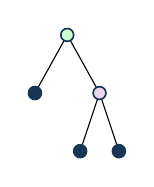
\begin{tikzpicture}[level distance=9mm,level 1/.style={sibling distance=10mm},level 2/.style={sibling distance=6mm},scale=.82,transform shape] \node[branch,fill=green!20] (n0) {} child {node[trueleaf] (n1) {}} child {node[branch,fill=violet!16] (n2) {} child {node[trueleaf] (n3) {}} child {node[trueleaf] (n4) {}}};\end{tikzpicture}\\[2pt]{\normalsize\texttt{\{1,\{1,1\}\}x100}}\end{minipage}\begin{minipage}[t]{.235\textwidth}\centering 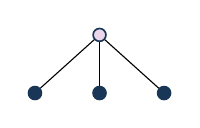
\begin{tikzpicture}[level distance=9mm,level 1/.style={sibling distance=10mm},level 2/.style={sibling distance=6mm},scale=.82,transform shape] \node[branch,fill=violet!16] (n0) {} child {node[trueleaf] (n1) {}} child {node[trueleaf] (n2) {}} child {node[trueleaf] (n3) {}};\end{tikzpicture}\\[2pt]{\normalsize\texttt{\{1,1,1\}x80}}\end{minipage}

{\footnotesize colored arity geometry; node color distinguishes constructors. Filled endpoints are true leaves; open endpoints are false/empty leaves. For colored grammars, color is genuine constructor data and is not silently converted into a positional zero pattern.}

{\footnotesize Typogeometric constructor codes and multiplicities: \(\Delta_{2}\!:\,5,\;\Delta_{3}\!:\,20,\;\Delta_{4}\!:\,40,\;\Delta_{5}\!:\,32\).}

\sectionbar{Coefficient and contour extraction}
{\footnotesize \[\begin{gathered}\mathcal K_n=\{(k_1,\ldots,k_4)\in\mathbb Z_{\ge0}^{4}:\sum_{j=1}^{4}jk_j=n-1\},\quad K=\sum_{j=1}^{4}k_j,\\a(n)=\frac{4}{n}\sum_{\boldsymbol k\in\mathcal K_n}\binom{n+K-1}{K}\binom{K}{k_1,\ldots,k_4}5^{k_1} 20^{k_2} 40^{k_3} 32^{k_4}.\end{gathered}\]}
\(a(n)=\dfrac{4}{2\pi i n}\oint_\gamma\dfrac{du}{\rho(u)^n},\quad n\ge1.\)

\sectionbar{Recurrence}
{\footnotesize \(\sum_{r=0}^{4}P_r(n)a(n+r)=0\) for \(n\ge 1\). The exact degree-4 coefficient polynomials are embedded in \texttt{certificate\_payload.json} (source: \texttt{release/certificate\_payload.json.gz\#/objects/p\_recurrence}).}

\sectionbar{Differential equation}
{\footnotesize The scalar linear ODE has order 4. It is obtained from the recurrence by the standard Euler-operator substitution. Exact coefficients and boundary polynomial: \texttt{release/certificate\_payload.json.gz\#/objects/ode\_from\_recurrence}.}

\sectionbar{Matrices, telescoper certificate, and checks}
{\small \(\text{No compact matrix tuple is shown; see the embedded exact reduction data.}\)}
\par\vspace{6pt}
{\small\textbf{Certificate.}\par\smallskip\(\displaystyle R(n,u)=N(n,u)/\rho(u)^{3},\ \deg_uN=16.\)\par}
\vspace{4pt}
{\small Telescoping identity: \(\sum_r P_r(n)H_{n+r}(u)=\partial_u\!\left(R(n,u)H_n(u)\right).\)\par}
\vspace{4pt}
{\footnotesize Matrix dimensions: \(10\times 10\); remainder \(4\times 5\), rank 4, nullity 1. The exact telescoping residual is zero. The recurrence reconstructs all 24 stored terms; 6/6 published OEIS prefix terms match.\par}

\vfill
\colorbox{soft}{\parbox{.97\textwidth}{\tiny Canonical records: \texttt{data/tree\_model.json}, \texttt{data/contour.json}, \texttt{data/matrices.json}, \texttt{data/recurrence.json}, \texttt{data/ode.json}. Embedded payload contains exact sources and SHA-256 matrix identifiers. Compare with the verbose certificate for A120590.}}
\end{document}
